\subsection{Données numériques aux redshifts clés}

Dans ce tableau, pour chaque redshift choisi \(z\in\{0,10,50,100,200,500,1000\}\), sont reportées les quantités normalisées suivantes :

\[
  R(z)
  =6\Bigl[2H^2(z)+(1+z)\,H(z)\,\frac{dH}{dz}\Bigr],
  \quad
  R_{0}
  =R(0)
  =6\Bigl[2H_{0}^{2}
    + H_{0}\,\frac{dH}{dz}\Bigl|_{z=0}\Bigr],
\]
\[
  f_{R}(R)
  =\frac{df}{dR},
  \quad
  f_{RR}(R)
  =\frac{d^{2}f}{dR^{2}},
  \quad
  m_{s}^{2}(R)
  =\frac{f_{R}(R)-R\,f_{RR}(R)}{3\,f_{RR}(R)},
\]
et l’indicateur
\[
  \mathrm{OK} \;=\;
    \begin{cases}
      1, & \text{si }f_{R}>0,\;f_{RR}>0,\;m_{s}^{2}>0,\\
      0, & \text{sinon.}
    \end{cases}
\]

\bigskip
Les valeurs numériques ont été obtenues de la manière suivante :

\begin{itemize}
  \item \(\displaystyle R(z)/R_{0}\) : extraction directe de la colonne \texttt{R\_over\_R0} dans \texttt{03\_r\_sur\_r0.csv}.
  \item \(f_{R}(R)\) et \(f_{RR}(R)\) : interpolation linéaire des colonnes \texttt{f\_R} et \texttt{f\_RR} de \texttt{03\_ricci\_fR\_exact.csv} aux valeurs de \(R/R_{0}\) extraites.
  \item \(m_{s}^{2}(R)/R_{0}\) : calcul analytique de \(m_{s}^{2}(R)\) selon la formule ci-dessus, puis division par \(R_{0}\).
\end{itemize}

\begin{table}[htbp]
  \centering
  \sisetup{
    table-number-alignment = center,
    round-mode            = places,
    round-precision       = 6,
    scientific-notation   = fixed
  }
  \caption{Valeurs numériques aux redshifts clés \(z\in\{0,10,50,100,200,500,1000\}\) :
    colonnes \(\,R(z)/R_{0}\) extraites de \texttt{03\_r\_sur\_r0.csv},
    \(f_{R}\) et \(f_{RR}\) interpolées depuis \texttt{03\_ricci\_fR\_exact.csv},
    puis \(m_{s}^{2}/R_{0}\) calculée analytiquement et normalisée par \(R_{0}\).
    OK = 1 si \(f_{R}>0\), \(f_{RR}>0\) et \(m_{s}^{2}>0\), sinon 0.}
  \label{tab:stabilite_fR_uniquement}
  \begin{tabular}{
    S[table-format=4.0]
    S[table-format=9.6]
    S[table-format=1.8]
    S[table-format=1.8]
    S[table-format=7.6]
    S[table-format=1]
  }
    \toprule
    { \(z\) } 
      & { \(\tfrac{R(z)}{R_{0}}\) } 
      & { \(f_{R}\) } 
      & { \(f_{RR}\) } 
      & { \(\tfrac{m_{s}^{2}}{R_{0}}\) } 
      & { OK } \\
    \midrule
    0    &    1.236430     & 1.00000000 & 0.00000100 &     6.114730 & 1 \\
    10   &  737.034100     & 1.00000900 & 0.00000100 &     5.605395 & 1 \\
    50   & 74342.277734    & 1.00000900 & 0.00000100 &     5.155319 & 1 \\
    100  &586685.022656    & 1.00000900 & 0.00000100 &     2.022478 & 1 \\
    200  &4770285.194738   & 1.00000900 & 0.00000100 &   -23.559133 & 0 \\
    500  &80660788.993320  & 1.00000900 & 0.00000100 &  -487.609504 & 0 \\
    1000 &733626464.373559 & 1.00000900 & 0.00000100 & -4480.322327 & 0 \\
    \bottomrule
  \end{tabular}
\end{table}

\subsubsection*{Tableau de contrôle rapide}

Le statut \texttt{OK}, qui signifie que toutes les conditions de stabilité linéaire 
(\(f_{R}>0\), \(f_{RR}>0\), \(m_{s}^{2}/R_{0}>0\)) sont satisfaites, reste à 1 pour 
\(z \le 200\) puis devient 0 pour \(z \ge 200\), signalant l’apparition d’instabilités linéaires au-delà de ce redshift.

\begin{table}[htbp]
  \centering
  \begin{tabular}{c c}
    \toprule
    Redshift \(z\) & OK \\
    \midrule
    0    & 1 \\
    10   & 1 \\
    50   & 1 \\
    100  & 1 \\
    200  & 0 \\
    500  & 0 \\
    1000 & 0 \\
    \bottomrule
  \end{tabular}
  \caption{Statut de stabilité linéaire : OK = 1 pour \(z \le 200\), OK = 0 pour \(z \ge 200\).}
  \label{tab:controle_rapide}
\end{table}

\subsection{Origine des données}

Les données numériques utilisées pour vérifier les conditions de stabilité linéaire proviennent des fichiers suivants :

\begin{itemize}
  \item \texttt{03\_ricci\_vs\_z.csv}  
    (colonnes \texttt{z}, \texttt{R\_over\_R0} – grille fine $0\le z\le1000$ par pas $\Delta z=1$,  
    où
    \[
    R(z)=6\bigl[2H^2(z)+(1+z)\,H(z)\,\tfrac{dH}{dz}\bigr]
    \]
    est calculé puis normalisé en \texttt{R\_over\_R0} = \(R(z)/R_0\).)
  \item \texttt{03\_ricci\_vs\_t.csv}  
    (colonnes \texttt{T\_Gyr}, \texttt{R\_over\_R0} – grille log–uniforme de l’âge cosmique $T$ en Gyr, où $R(T)$ est calculé et normalisé par $R_0$, utilisée pour le calcul de l’invariant adimensionnel  
    \[
     I_{3}(T) \;=\; f_{R}\bigl(R(T)\bigr)\;-\;1
    \]
    via interpolation sur \texttt{03\_ricci\_fR\_exact.csv}.)  
  \item \texttt{03\_ricci\_fR\_exact.csv}  
    (colonnes \texttt{R\_over\_R0}, \texttt{f\_R}, \texttt{f\_RR} – grille $R/R_0\in[0,10]$ par pas de $0{,}1$,  
    interpolation linéaire (via \texttt{numpy.interp}) des valeurs de \(f_R\) et \(f_{RR}\)  
     pour les paramètres de référence $\beta=10^{-6}$, $\gamma=5\times10^{-9}$.)
  \item \texttt{03\_r\_sur\_r0.csv}  
    (colonnes \texttt{z}, \texttt{R\_over\_R0} – extrait interpolé aux redshifts clés $\{0,10,50,100,200,500,1000\}$, arrondi à 6 décimales)
  \item \texttt{03\_stabilite\_fR\_frontiere.csv}  
    (colonnes \texttt{beta}, \texttt{gamma}, \texttt{OK} – liste des couples $(\beta,\gamma)$ à la frontière où OK passe de 1 à 0)
  \item \texttt{03\_stabilite\_fR\_domaine.csv}  
    (colonnes \texttt{beta}, \texttt{gamma}, \texttt{OK} – grille log–log de $(\beta,\gamma)$ avec OK=1 stable, incluant explicitement le point de référence $(10^{-6},5\times10^{-9})$)
\end{itemize}

La colonne \texttt{OK} (valeur 0 ou 1) dans chaque CSV signale la validation numérique simultanée de
\[
  f_{R}(R)>0,\quad f_{RR}(R)>0,\quad \frac{m_{s}^{2}(R)}{R_{0}}>0
\]
pour les redshifts considérés.  

\subsection{Graphiques clés}

Les deux figures suivantes sont générées par le script \texttt{13\_tracer\_stabilite\_fR.py} 
à partir des mêmes sources CSV.

\subsubsection*{Figure 02 : $f_{R}(R)$ et $f_{RR}(R)$ en fonction de $R/R_{0}$}

\begin{figure}[htbp]
  \centering
  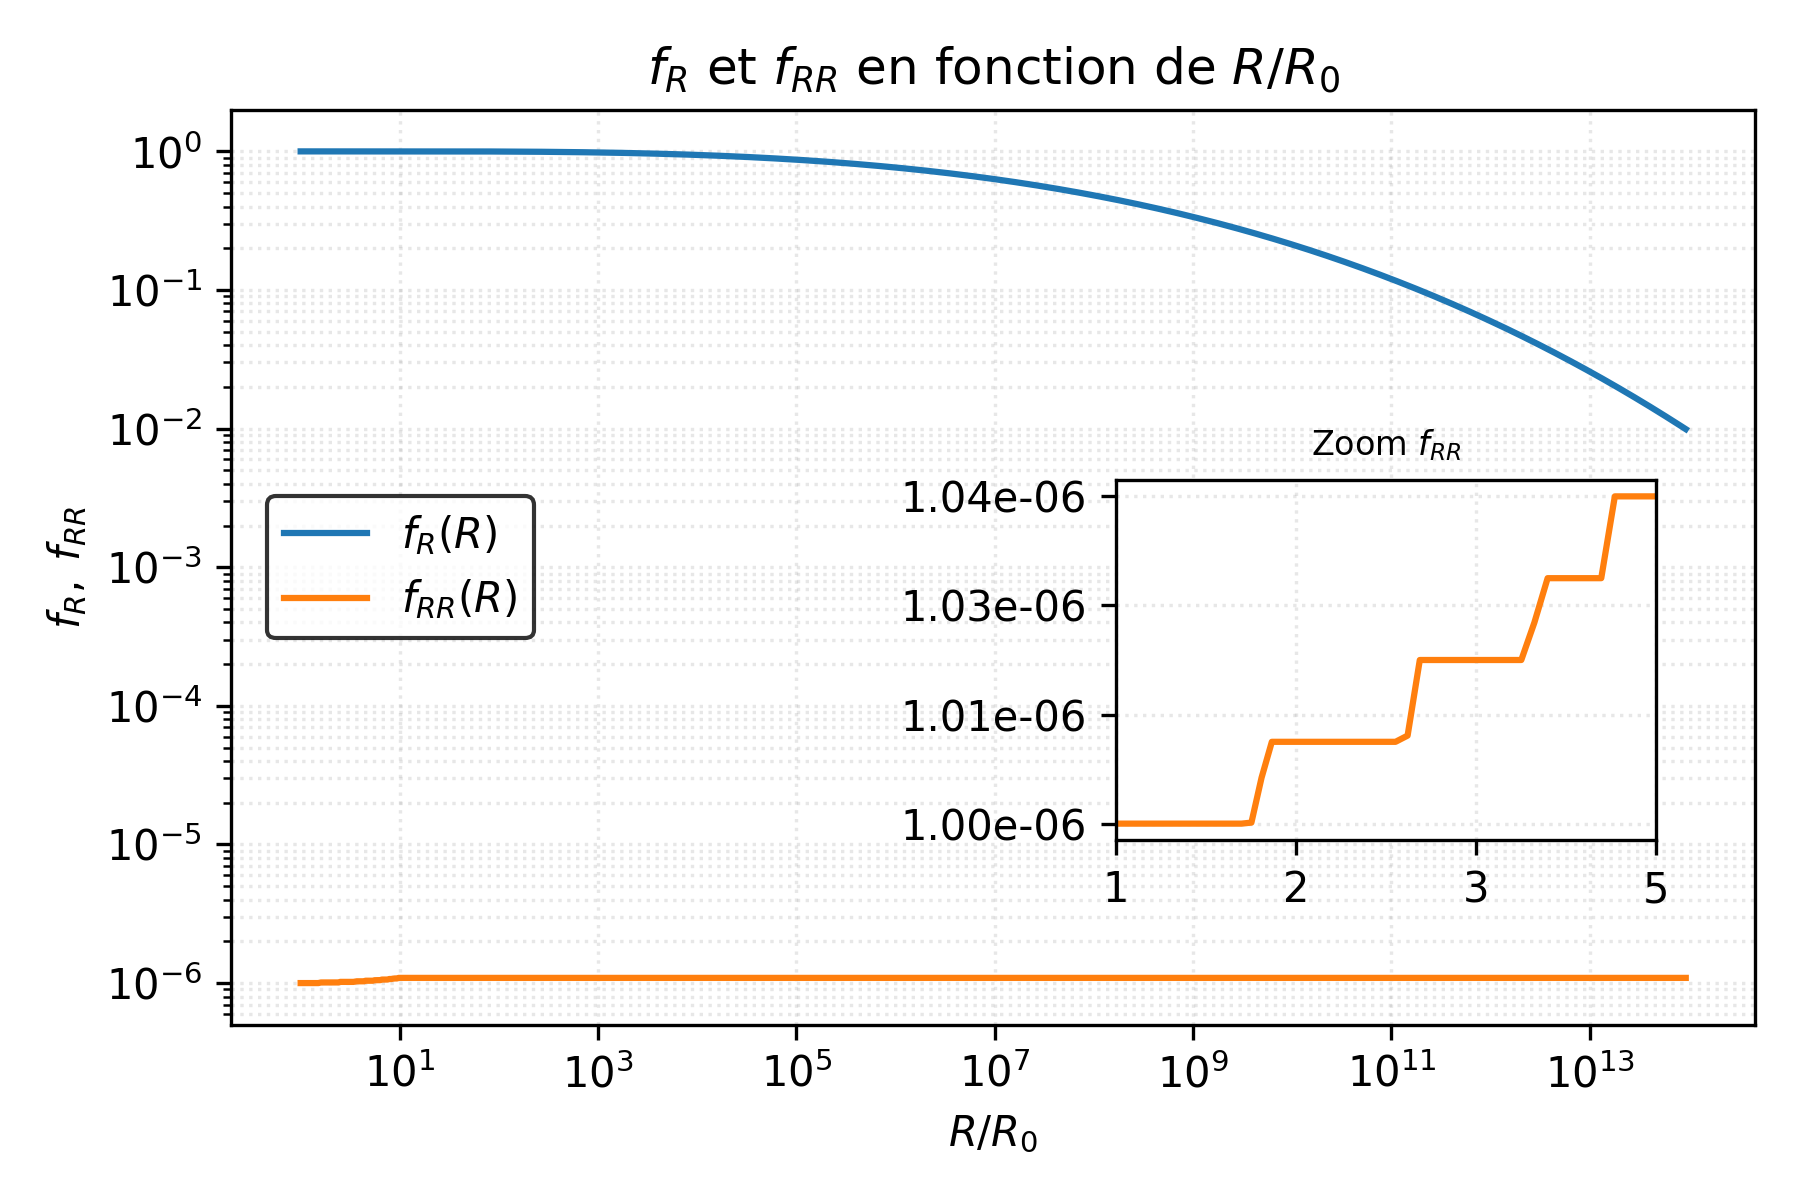
\includegraphics[width=0.75\textwidth]{03-stabilite-fR/fig_02_fR_fRR_vs_R.png}
  \caption{Tracé en échelles log–log de $f_{R}(R)$ (ocre) et $f_{RR}(R)$ (orange)  
    en fonction de $R/R_{0}$ sur l’intervalle $[10^{-1},\,10^{1}]$, données issues de \texttt{03\_ricci\_fR\_exact.csv}.  
    On constate que $f_{R}(R)\gtrsim1$ et que $f_{RR}(R)>0$ sur toute la plage considérée.}
  \label{fig:fR_fRR_vs_R}
\end{figure}

\subsubsection*{Figure 03 : Évolution zoomée de $m_{s}^{2}(z)/R_{0}$}

\begin{figure}[htbp]
  \centering
  \includegraphics[width=0.75\textwidth]{03-stabilite-fR/fig_03_ms2_vs_z.png}
  \caption{Zoom sur l’évolution de $m_{s}^{2}(z)/R_{0}$ (ordonnée en échelle log)  
    pour $0\le z\le60$. Données interpolées à partir de \texttt{03\_ricci\_vs\_z.csv}  
    et \texttt{03\_ricci\_fR\_exact.csv}. On constate que $m_{s}^{2}/R_{0}$  
    reste strictement positif pour $z\le60$, puis décline rapidement à plus grand $z$,  
    indiquant la transition vers des instabilités linéaires.}
  \label{fig:ms2_vs_z}
\end{figure}

\noindent\emph{Script : \texttt{13\_tracer\_stabilite\_fR.py}.}

\subsection{Vérification numérique des conditions de stabilité}

Les résultats du tableau~\ref{tab:stabilite_fR_uniquement} et des figures
\ref{fig:fR_fRR_vs_R} et \ref{fig:ms2_vs_z} confirment que :

\begin{itemize}
  \item Pour tous les redshifts clés $z\in\{0,10,50,100,200,500,1000\}$, on a
    \[
      f_{R}\bigl(R(z)\bigr)>0
      \quad\text{et}\quad
      f_{RR}\bigl(R(z)\bigr)>0,
    \]
    assurant l’absence de ghost et la convexité de $f(R)$ sur $0 \le z \le 1000$.
  \item La condition
    \[
      \frac{m_{s}^{2}\bigl(R(z)\bigr)}{R_{0}}>0
    \]
    est satisfaite pour $z \le 100$ et devient négative pour $z \ge 200$, signalant l’apparition d’instabilités linéaires à partir de $z=200$.
\end{itemize}

La colonne \texttt{OK} du tableau indique cette validation numérique : OK = 1 si et seulement si les trois inégalités sont simultanément vérifiées, OK = 0 sinon.

\subsection{Conclusion détaillée}

L’analyse numérique des redshifts clés $z\in\{0,10,50,100,200,500,1000\}$ révèle :

\begin{itemize}
  \item Les deux premières conditions de stabilité,
    \[
      f_{R}(R)>0
      \quad\text{et}\quad
      f_{RR}(R)>0,
    \]
    sont vérifiées sur tout l’intervalle $0\le z\le1000$, garantissant l’absence de ghost et la convexité de $f(R)$.
  \item La troisième condition,
    \[
      \frac{m_{s}^{2}(R)}{R_{0}}>0,
    \]
    est satisfaite pour $z\le100$ et devient négative pour $z\ge200$, signalant l’apparition d’instabilités linéaires à partir de $z=200$.
\end{itemize}

Ces résultats, fondés sur les fichiers
\texttt{03\_ricci\_vs\_z.csv} et
\texttt{03\_ricci\_fR\_exact.csv} et illustrés par les figures~\ref{fig:fR_fRR_vs_R}
et~\ref{fig:ms2_vs_z},
montrent que l’extension $f(R)$, paramétrée par
$\beta=10^{-6}$ et $\gamma=5\times10^{-9}$, reste linéairement stable pour
$0\le z\le100$ et présente des instabilités pour $z\ge200$.

\subsubsection*{Transition vers le Chapitre 4}

Ayant établi le bilan de stabilité linéaire, l’étape suivante consiste à étudier
les invariants adimensionnels $I_{1}(T)$, $I_{2}(T)$ et $I_{3}(T)$, qui
seront présentés au Chapitre 4.

\subsubsection*{Limites et perspectives}

Bien que l’extension $f(R)$ soit stable pour $0\le z\le100$, plusieurs axes
méritent approfondissement :

\begin{itemize}
  \item \textbf{Ordres supérieurs de la série :}
    l’ajout de termes $(R-R_{0})^n$ pour $n>3$ pourrait affecter la stabilité à haut~$z$.
  \item \textbf{Contraintes non linéaires :}
    l’étude des instabilités non linéaires ou résonances en champ fort reste à faire.
  \item \textbf{Couplages à la matière :}
    l’impact des couplages sombre ou standard sur $f_R$ et~$m_s^2$ localement.
  \item \textbf{Tests observationnels :}
    comparaison aux données de croissance de structures et de lentilles gravitationnelles.
  \item \textbf{Optimisation des performances :}
    maillage adaptatif en $z$ et méthodes d’intégration avancées.
\end{itemize}

\subsection*{Glossaire}

\begin{itemize}
  \item \(\,R(z)\) : scalaire de Ricci, fonction du redshift \(z\) donnée par  
    \[
      R(z)
      =6\Bigl[2H^2(z)+(1+z)\,H(z)\,\frac{dH}{dz}\Bigr],
    \]
    avec \(H(z)\) la fonction de Hubble.
  \item \(R_{0}\) : scalaire de Ricci au redshift \(z=0\), défini et       utilisé dans sa forme simplifiée pour \(\Lambda\)CDM sans              contribution radiation :  
    \[
    R_{0} \;\equiv\; R(0) \;=\; 12\,H_{0}^{2},
    \]
    ce qui correspond à l’approximation 
    \(\tfrac{dH}{dz}\bigl|_{z=0}\approx -\tfrac{3}{2}\,H_{0}\,\Omega_{m}\approx0\) 
    dans un univers dominé par la constante cosmologique et la matière.  
    Cette valeur est employée de façon cohérente dans tous les calculs et CSV associés.
  \item \(\beta,\;\gamma\) : paramètres fixes de l’extension \(f(R)\), choisis typiquement  
    \(\beta=10^{-6},\;\gamma=5\times10^{-9}.\)
  \item \(f(R)\) : fonction gravitationnelle modifiée,  
    \[
      f(R)
      =R
      +\frac{\beta}{2\,R_{0}}\,(R-R_{0})^{2}
      +\frac{\gamma}{3\,R_{0}^{2}}\,(R-R_{0})^{3}.
    \]
  \item \(f_{R}(R)\) : première dérivée de \(f\) par rapport à \(R\),  
    \[
      f_{R}(R)=\frac{df}{dR}.
    \]
  \item \(f_{RR}(R)\) : seconde dérivée de \(f\),  
    \[
      f_{RR}(R)=\frac{d^{2}f}{dR^{2}}.
    \]
  \item \(m_{s}^{2}(R)\) : masse scalaire associée,  
    \[
      m_{s}^{2}(R)
      =\frac{f_{R}(R)-R\,f_{RR}(R)}{3\,f_{RR}(R)}.
    \]
  \item \(z\) : redshift, paramètre décrivant l’échelle cosmologique.
  \item \(\mathrm{OK}\) : indicateur (0 ou 1) signalant que simultanément  
    \(f_{R}(R)>0\), \(f_{RR}(R)>0\) et \(m_{s}^{2}(R)/R_{0}>0\).
\end{itemize}

\bigskip
\noindent\emph{Fin de la partie détaillée, Chapitre 3.}